% Options for packages loaded elsewhere
\PassOptionsToPackage{unicode}{hyperref}
\PassOptionsToPackage{hyphens}{url}
%

%%% Setup
\documentclass[12pt,a4paper]{article}
\title{Project Documentation}
\author{Team Duck Duck Go}
\date{} %no date if empty, current date if commented out

\usepackage{minted}

%%%%% Auto generated by pandoc %%%%%

\usepackage{amsmath,amssymb}
\usepackage{lmodern}
\usepackage{iftex}
\ifPDFTeX
  \usepackage[T1]{fontenc}
  \usepackage[utf8]{inputenc}
  \usepackage{textcomp} % provide euro and other symbols
\else % if luatex or xetex
  \usepackage{unicode-math}
  \defaultfontfeatures{Scale=MatchLowercase}
  \defaultfontfeatures[\rmfamily]{Ligatures=TeX,Scale=1}
\fi
% Use upquote if available, for straight quotes in verbatim environments
\IfFileExists{upquote.sty}{\usepackage{upquote}}{}
\IfFileExists{microtype.sty}{% use microtype if available
  \usepackage[]{microtype}
  \UseMicrotypeSet[protrusion]{basicmath} % disable protrusion for tt fonts
}{}
\makeatletter
\@ifundefined{KOMAClassName}{% if non-KOMA class
  \IfFileExists{parskip.sty}{%
    \usepackage{parskip}
  }{% else
    \setlength{\parindent}{0pt}
    \setlength{\parskip}{6pt plus 2pt minus 1pt}}
}{% if KOMA class
  \KOMAoptions{parskip=half}}
\makeatother
\usepackage{xcolor}
\usepackage{longtable,booktabs,array}
\usepackage{calc} % for calculating minipage widths
% Correct order of tables after \paragraph or \subparagraph
\usepackage{etoolbox}
\makeatletter
\patchcmd\longtable{\par}{\if@noskipsec\mbox{}\fi\par}{}{}
\makeatother
% Allow footnotes in longtable head/foot
\IfFileExists{footnotehyper.sty}{\usepackage{footnotehyper}}{\usepackage{footnote}}
\makesavenoteenv{longtable}
\usepackage{graphicx}
\makeatletter
\def\maxwidth{\ifdim\Gin@nat@width>\linewidth\linewidth\else\Gin@nat@width\fi}
\def\maxheight{\ifdim\Gin@nat@height>\textheight\textheight\else\Gin@nat@height\fi}
\makeatother
% Scale images if necessary, so that they will not overflow the page
% margins by default, and it is still possible to overwrite the defaults
% using explicit options in \includegraphics[width, height, ...]{}
\setkeys{Gin}{width=\maxwidth,height=\maxheight,keepaspectratio}
% Set default figure placement to htbp
\makeatletter
\def\fps@figure{htbp}
\makeatother
\setlength{\emergencystretch}{3em} % prevent overfull lines
\providecommand{\tightlist}{%
  \setlength{\itemsep}{0pt}\setlength{\parskip}{0pt}}
\setcounter{secnumdepth}{-\maxdimen} % remove section numbering
\ifLuaTeX
  \usepackage{selnolig}  % disable illegal ligatures
\fi
\IfFileExists{bookmark.sty}{\usepackage{bookmark}}{\usepackage{hyperref}}
\IfFileExists{xurl.sty}{\usepackage{xurl}}{} % add URL line breaks if available
\urlstyle{same} % disable monospaced font for URLs
\hypersetup{
  hidelinks,
  pdfcreator={LaTeX via pandoc}}


%%%%% End pandoc stuff %%%%%

\begin{document}


\maketitle
\section{Introduction} % do \section*{} to remove numbering


This web application prototype is designed to retrieve information on
Single Nucleotide Polymorphisms (SNPs) seen in Type 1 Diabetes patients
identified by Genome wide association studies (GWAS). The database will
use information from the GWAS catalogue, along with population data from
Ensembl and the 1000 Genomes Project and functional information and Gene
Ontology information obtained through Ensembl's VEP tool which is all is
retrievable through a user friendly interface through the input of an
rsID, Chromosome position or a Gene name. The site also allows the user
to calculate Linkage Disequilibrium (LD) of SNPs selected for each
population producing a text file containing the LD values and plot these
values as a LD heatmap. The user is also able to enter multiple SNPs and
return a Manhattan plot of the p-values.

\subsection{Prerequisites:}


\subsubsection{Functions used throughout:}

A number of functions were used throughout the code such as \ldots{}


\inputminted{python}{code_snippets/db_scripts1.py}


\protect\hypertarget{t.a725f3f15ee101df28c7684965a6bd8a25eed434}{}{}\protect\hypertarget{t.1}{}{}

\begin{longtable}[]{@{}
  >{\raggedright\arraybackslash}p{(\columnwidth - 0\tabcolsep) * \real{1.0000}}@{}}
\toprule()
\endhead
\begin{minipage}[t]{\linewidth}\raggedright
{~ ~naughtyList={[}{]} ~ ~ ~ ~ ~ ~ ~ ~ ~ ~ ~ ~ ~ ~ ~ ~ ~}{\# List of
lists of (index, p-val) we want to drop}{\hfill\break
~ }{for}{~i }{in}{~dupesDict:\\
\hspace*{0.333em} ~ ~ snp = dupesDict{[}i{]} ~ ~ ~ ~ ~ ~ ~ ~ ~ ~ ~ ~
~}{\# Get list of (index, pVal)}{\hfill\break
~ ~ ~ sortByP=sorted(snp,key=}{lambda}{~x: }{0}{-x{[}}{1}{{]}) ~ ~}{\#
Sort by p-value}{\hfill\break
~ ~ ~ sortByP=sortByP{[}}{1}{:{]} ~ ~ ~ ~ ~ ~ ~ ~ ~ ~ ~ ~ }{\# Select
all but greatest p value}{\hfill\break
~ ~ ~ naughtyList.append(sortByP)\\
\strut \\
\strut \\
\hspace*{0.333em} dropList={[}{]} ~ ~ ~ ~ ~ ~ ~ ~ ~ ~ ~ ~ }{\# List of
indices for rows we want to drop}{\hfill\break
~ }{for}{~i }{in}{~naughtyList: ~ ~ ~ ~ ~ ~ ~ }{\# Enter first
list}{\hfill\break
~ ~ ~ }{for}{~j }{in}{~i: ~ ~ ~ ~ ~ ~ ~ ~ ~ ~ }{\# Enter second
list}{\hfill\break
~ ~ ~ ~ ~ dropList.append(j{[}}{0}{{]}) ~ ~ ~ }{\# Add the index from
each tuple}{\hfill\break
\hfill\break
\hfill\break
~ }{return}{(dataframe.drop(dropList)) ~ ~}{\# Return dataframe without
duplicate values}\strut
\end{minipage} \\
\bottomrule()
\end{longtable}

{\hfill\break
\hfill\break
\hfill\break
}

\protect\hypertarget{t.59b2d73cce28e0f846926b398a5396f1238f472c}{}{}\protect\hypertarget{t.2}{}{}

\begin{longtable}[]{@{}
  >{\raggedright\arraybackslash}p{(\columnwidth - 0\tabcolsep) * \real{1.0000}}@{}}
\toprule()
\endhead
\begin{minipage}[t]{\linewidth}\raggedright
{def}{~removeDupeGeneMap(GeneMap):\\
\hspace*{0.333em} }{try}{:\\
\hspace*{0.333em} ~ ~ GeneMap=GeneMap.split(}{\textquotesingle,
\textquotesingle{}}{)\\
\hspace*{0.333em} ~ ~ uniques=}{""}{\hfill\break
~ ~ ~ }{for}{~item }{in}{~GeneMap:\\
\hspace*{0.333em} ~ ~ ~ ~ }{if}{~item }{not}{~}{in}{~uniques: }{\# If
the item hasn\textquotesingle t been seen before,}{\hfill\break
~ ~ ~ ~ ~ ~ ~ uniques+=(item) ~ ~ }{\# add it to the list.}{\hfill\break
~ ~ ~ ~ ~ ~ ~ uniques+=(}{", "}{) ~ ~ }{\# Also add \textquotesingle{}
,\textquotesingle{}}{\hfill\break
~ ~ ~ }{return}{~(uniques{[}:}{-2}{{]}) ~ ~ ~ }{\# Remove last
\textquotesingle{} ,\textquotesingle{}}{\hfill\break
~ }{except}{:\\
\hspace*{0.333em} ~ ~ }{return}{~(}{"Data unavailable"}{) ~ ~ }{\#
Return this if geneMap is empty}\strut
\end{minipage} \\
\bottomrule()
\end{longtable}

\hypertarget{h.vhchvtb4vp8x}{%
\subsection{\texorpdfstring{{}}{}}\label{h.vhchvtb4vp8x}}

\hypertarget{h.exepwhhdz8ou}{%
\subsection{\texorpdfstring{{Structure:}}{Structure:}}\label{h.exepwhhdz8ou}}

{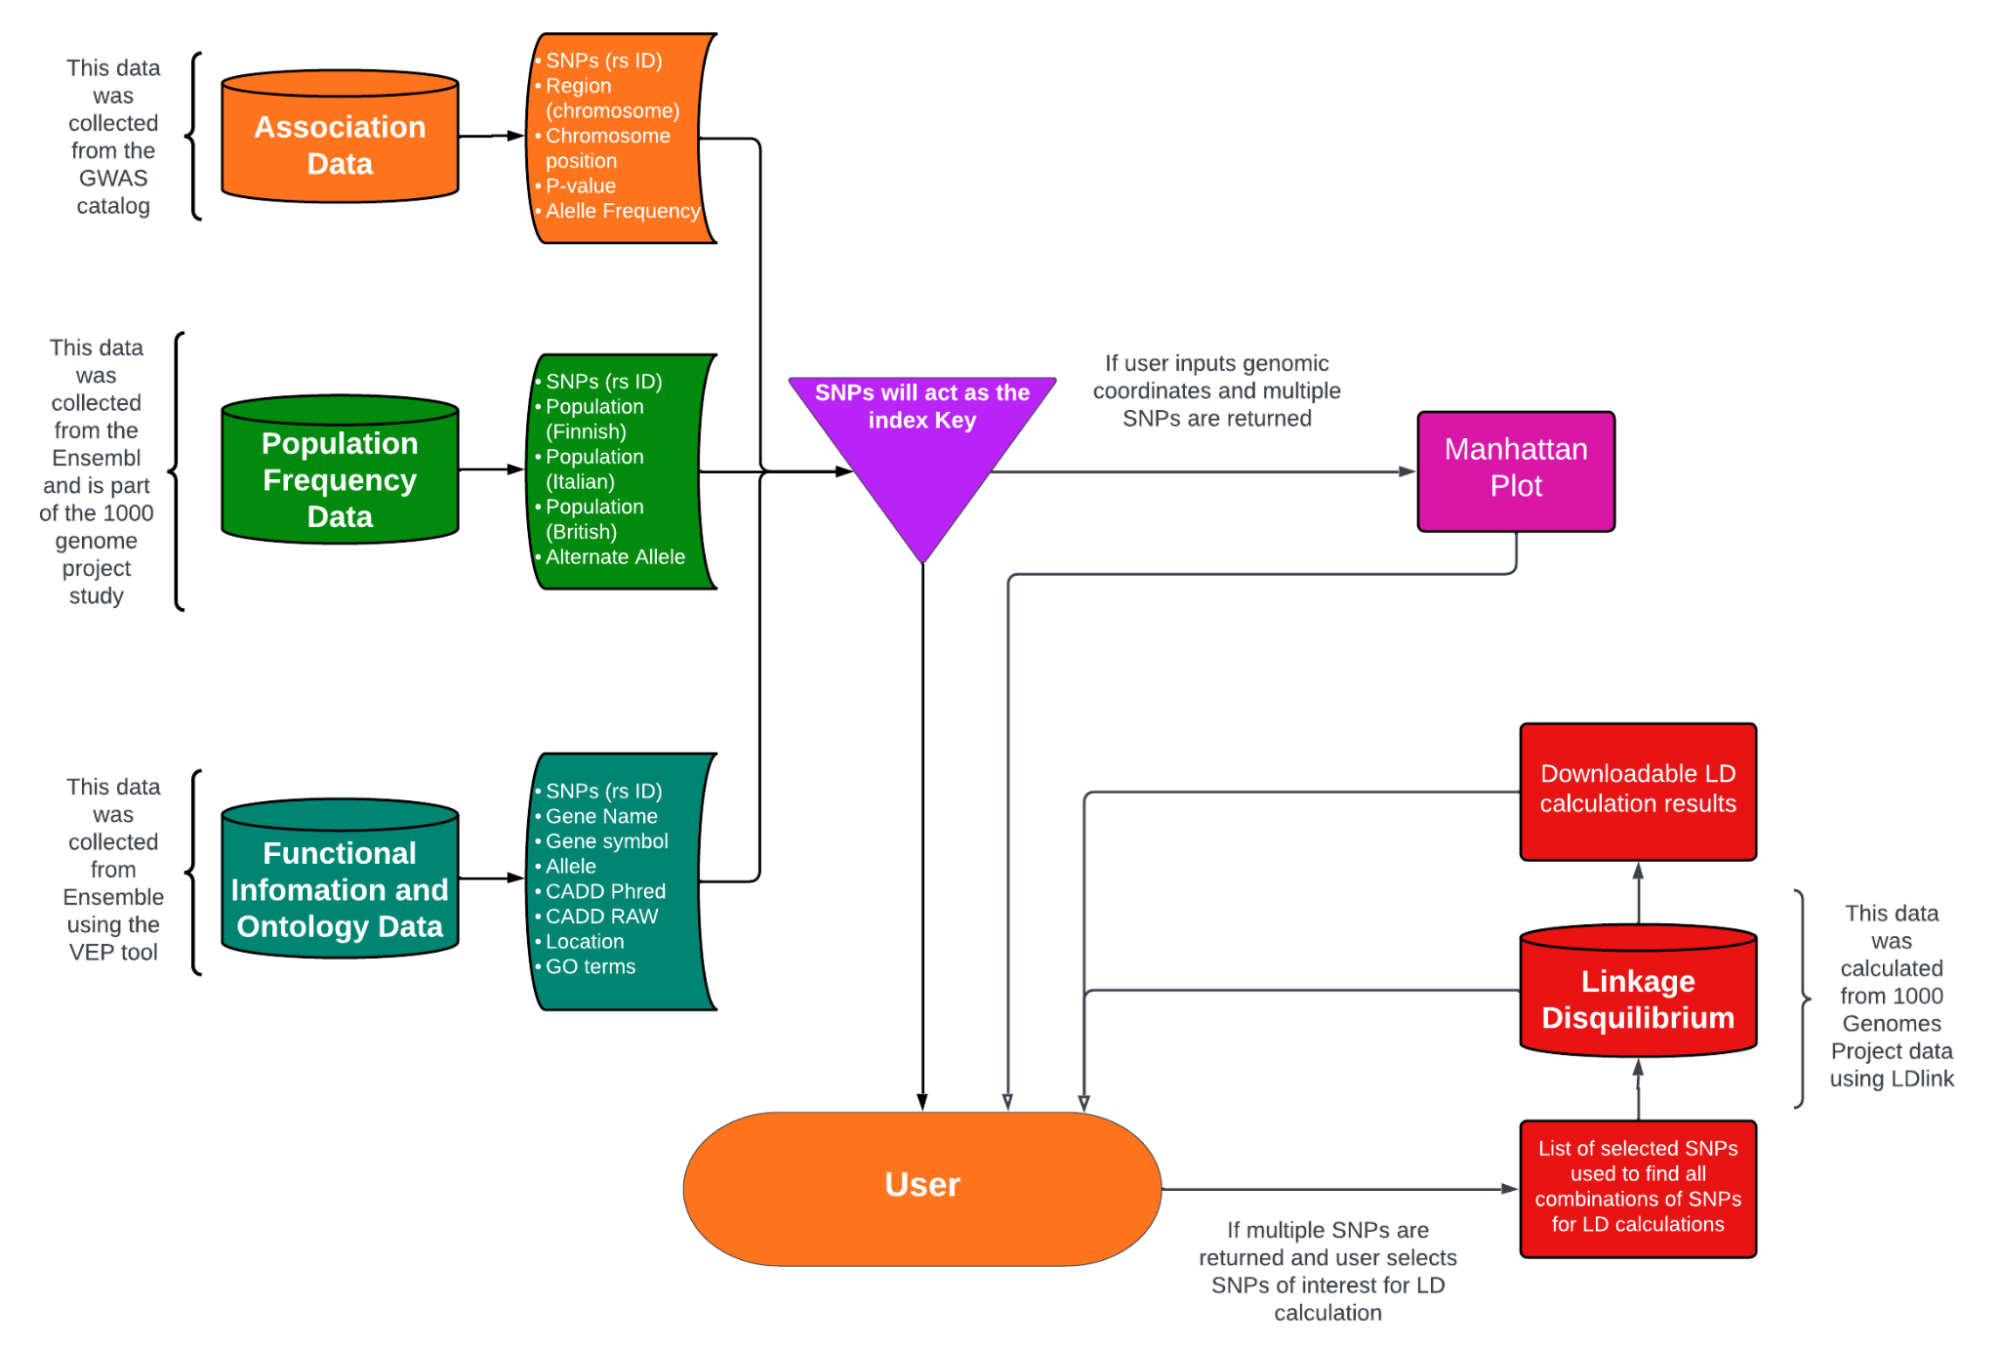
\includegraphics{images/image4.png}}

{}

\hypertarget{h.9yfmc6qy2clu}{%
\subsubsection{\texorpdfstring{{GWAS:}}{GWAS:}}\label{h.9yfmc6qy2clu}}

{This information was downloaded from the GWAS catalogue where a TSV
file was downloaded and then trimmed using the following code;}

\protect\hypertarget{t.b1af7d7bc328582cfe763ff0e0cbb9d8bcbeb335}{}{}\protect\hypertarget{t.3}{}{}

\begin{longtable}[]{@{}
  >{\raggedright\arraybackslash}p{(\columnwidth - 0\tabcolsep) * \real{1.0000}}@{}}
\toprule()
\endhead
\begin{minipage}[t]{\linewidth}\raggedright
{fileIn =
getPath(}{\textquotesingle gwas\_catalog\_v1.0-associations\_e108\_r2023-01-14.tsv\textquotesingle{}}{)
}{\# https://www.ebi.ac.uk/gwas/docs/file-downloads}{\hfill\break
fileOut =
getPath(}{\textquotesingle gwas\_trimmed.tsv\textquotesingle{}}{)\\
\strut \\
data = pd.read\_csv(fileIn,
sep=}{\textquotesingle\textbackslash t\textquotesingle{}}{,
low\_memory=}{False}{) ~ ~}{\# Reads gwas tsv}{\hfill\break
data=removeSpecial(data) ~ ~}{\# removes special characters in column
names}\strut
\end{minipage} \\
\bottomrule()
\end{longtable}

{This code uses pandas to open the TSV file, creates a dataframe called
data, and removes any special characters from the column names, as SQL
does not interact with special characters very well.}

\protect\hypertarget{t.638fb5b406f87bace7364f8ea9275d9a6c56f7f3}{}{}\protect\hypertarget{t.4}{}{}

\begin{longtable}[]{@{}
  >{\raggedright\arraybackslash}p{(\columnwidth - 0\tabcolsep) * \real{1.0000}}@{}}
\toprule()
\endhead
\begin{minipage}[t]{\linewidth}\raggedright
{data=data.query(}{"disease\_trait==\textquotesingle Type 1
diabetes\textquotesingle{} or study.str.contains(\textquotesingle type 1
diabetes\textquotesingle)"}{)\\
data =
data.loc{[}data.snps.str.contains(}{r\textquotesingle rs{[}0-9{]}+\textquotesingle{}}{){]}
~ ~ ~ ~}{\# get only snps with rsids}{\hfill\break
}{\#data =
data.loc{[}data{[}\textquotesingle CHR\_ID\textquotesingle{]}==\textquotesingle6\textquotesingle{]}
~ ~ ~ ~ ~ ~ ~ ~ ~ ~ ~ ~\# Select only rows for chromosome 6}\strut
\end{minipage} \\
\bottomrule()
\end{longtable}

{The data frame is then filtered further so that it only has data that
references T1D in the ``disease\_trait'' column so that only T1D data
remains in the dataframe. Next all SNPs that don\textquotesingle t have
rsIDs are removed, as some cells had incompatible data in this column.}

\protect\hypertarget{t.132f647eb56f42c8d7dbb1fffca78301f723bdb3}{}{}\protect\hypertarget{t.5}{}{}

\begin{longtable}[]{@{}l@{}}
\toprule()
\endhead
{data =
data{[}{[}}{"snps"}{,}{"region"}{,}{"chr\_pos"}{,}{"chr\_id"}{,}{"p\_value"}{,}{"mapped\_gene"}{{]}{]}} \\
\bottomrule()
\end{longtable}

{The da}{taframe is then trimmed again so that it contains only the
columns of interest ~ "snps", "region", "chr\_pos", "chr\_id",
"p\_value", "mapped\_gene". }

{}

\protect\hypertarget{t.8adbe8fae2f67de92759b4b70695249a62c02e6d}{}{}\protect\hypertarget{t.6}{}{}

\begin{longtable}[]{@{}
  >{\raggedright\arraybackslash}p{(\columnwidth - 0\tabcolsep) * \real{1.0000}}@{}}
\toprule()
\endhead
\begin{minipage}[t]{\linewidth}\raggedright
{data=removeDupeSNP(data) ~ ~}{\# Remove duplicates (leaving the entry
with largest p value)}{\hfill\break
newCol={[}removeDupeGeneMap(r{[}}{"mapped\_gene"}{{]}) }{for}{~i, r
}{in}{~data.iterrows(){]}}

{data{[}}{"mapped\_gene"}{{]}=newCol}\strut
\end{minipage} \\
\bottomrule()
\end{longtable}

{Duplicate mapped\_gene information is then removed.}

{}

\protect\hypertarget{t.efbc0c483d3f71e27abdb0a27605856edba6693c}{}{}\protect\hypertarget{t.7}{}{}

\begin{longtable}[]{@{}
  >{\raggedright\arraybackslash}p{(\columnwidth - 0\tabcolsep) * \real{1.0000}}@{}}
\toprule()
\endhead
\begin{minipage}[t]{\linewidth}\raggedright
{data.rename(columns =
\{}{\textquotesingle snps\textquotesingle{}}{:}{\textquotesingle rsid\textquotesingle{}}{\},
inplace = }{True}{)\\
\strut \\
}{\# if os.path.exists(fileOut): \# If the file exists,}{\hfill\break
}{\# ~ ~ os.remove(fileOut) ~ ~ \# delete it.}{\hfill\break
data.to\_csv(fileOut,
sep=}{\textquotesingle\textbackslash t\textquotesingle{}}{,
index=}{False}{)}\strut
\end{minipage} \\
\bottomrule()
\end{longtable}

{Next the column \textquotesingle snps\textquotesingle{} was renamed to
\textquotesingle rsid\textquotesingle{} and made the change directly to
the dataframe by setting inplace=True.}

\hypertarget{h.o8avd7mg5nfg}{%
\subsubsection{\texorpdfstring{{Functional information and Gene
Ontology:}}{Functional information and Gene Ontology:}}\label{h.o8avd7mg5nfg}}

{We have used Ensembl\textquotesingle s Variant Effect Predictor web
tool to gather the Functional and Ontology data by submitting a job with
the rsIDs as input from the above GWAS TSV file. After running the job,
we get an output of text file with columns like:}

{rsid: the reference SNP identifier for the variant.}

{Allele: the alternative allele observed at the variant site.}

{impact: the impact of the variant on the affected gene}

{consequence: the consequence of the variant on the affected gene}

{location: the location of the variant within the affected gene}

{Gene: the Ensembl gene ID of the affected gene.}

{Symbol: the gene symbol or name.}

{Feature\_Type: the type of genomic feature the variant is located in}

{Feature: the Ensembl ID of the specific feature the variant is located
in}

{Exon: the exon number(s) affected by the variant.}

{Intron: the intron number(s) affected by the variant.}

{HGVSc: the HGVS nomenclature for the variant at the cDNA .}

{HGVSp: the HGVS nomenclature for the variant at the protein level.}

{cDNA\_position: the position of the variant within the cDNA sequence of
the affected gene.}

{CDS\_position: the position of the variant within the coding sequence
of the affected gene.}

{Protein\_position: the position of the variant within the protein
sequence of the affected gene.}

{Amino\_acids: the amino acid change resulting from the variant.}

{Codons: the DNA codon change resulting from the variant.}

{Existing\_variation: additional identifiers for the variant in other
databases.}

{Distance: the distance to the nearest feature in the same or opposite
strand.}

{Strand: the genomic strand the variant is located on.}

{FLAGS: additional information about the variant .}

{SYMBOL\_SOURCE: the source of the gene symbol or name.}

{HGNC\_ID: the HGNC gene ID of the affected gene.}

{MANE\_SELECT: indication of whether this transcript is the MANE
(Matched Annotation from NCBI and EMBL-EBI) Select transcript.}

{MANE\_PLUS\_CLINICAL: indication of whether this transcript is the MANE
Select Plus Clinical (MPC) transcript.}

{TSL: transcript support level (a measure of transcript annotation
confidence).}

{APPRIS: annotation of principal isoforms for each gene.}

{ENSP: the Ensembl protein ID of the affected protein.}

{SIFT: prediction of the effect of the variant on protein function.}

{PolyPhen: prediction of the effect of the variant on protein function.}

{CLIN\_SIG: clinical significance of the variant.}

{SOMATIC: indication of whether the variant is somatic or germline.}

{PHENO: phenotype association of the variant.}

{PUBMED: PubMed ID of publications reporting functional evidence of the
variant.}

{MOTIF\_NAME: name of the DNA motif affected by the variant.}

{MOTIF\_POS: position of the variant within the affected DNA motif.}

{HIGH\_INF\_POS: indication of whether the variant falls in a highly
conserved position within the DNA motif.}

{MOTIF\_SCORE\_CHANGE: the effect of the variant on the score of the
affected DNA motif.}

{TRANSCRIPTION\_FACTORS: transcription factors that bind the affected
DNA motif.}

{CADD\_PHRED: Phred-scaled CADD score (Combined Annotation-Dependent
Depletion), which predicts the deleteriousness of variants.}

{CADD\_RAW: the raw CADD score, which is a measure of the
deleteriousness of variants.}

{GO Terms: Gene Ontology (GO) terms associated with the affected gene.}

{The VEP file provides detailed information about the functional and
ontological consequences of genetic variants, including their impact on
genes, proteins, and pathways.}

{We have converted the text file to a tsv file and trimmed down the file
to include only the rsID, Alleles, CADD\_PHRED and CADD\_RAW scores
columns for the functional data and the rsID, location, gene, symbol, GO
terms columns for the Ontology data. We have further used these TSV
files in our database.}

{CADD (Combined Annotation Dependent Depletion) is a tool used for
predicting the potential harm caused by genetic variants. The tool
generates a score that indicates the likelihood of a variant being
deleterious.}

{One advantage of CADD over SIFT and PolyPhen is that CADD integrates a
larger and more diverse set of functional annotations. It also considers
the effects of variants on non-coding regions of the genome, which can
be important for understanding the functional consequences of variants
that are not in protein-coding regions.}

{}

\begin{center}\rule{0.5\linewidth}{0.5pt}\end{center}

\hypertarget{h.bob8u1u023ib}{%
\subsubsection{\texorpdfstring{{}}{}}\label{h.bob8u1u023ib}}

\hypertarget{h.x88z4oadkpbf}{%
\subsubsection{\texorpdfstring{{Linkage
Disequilibrium:}}{Linkage Disequilibrium:}}\label{h.x88z4oadkpbf}}

{Linkage disequilibrium (LD) is the degree of non-random association of
the allele of one SNP with the allele of another SNP within a
population. LD is typically measured by two metrics: D' and r}{2}{. }

{D' is the normalised values of D, the coefficient of linkage
disequilibrium, where A and B are alleles of two SNPs in different
loci:}

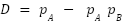
\includegraphics{images/image1.png}{~}

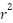
\includegraphics{images/image2.png}{~ }{is the correlation coefficient
between two loci:}

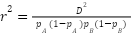
\includegraphics{images/image3.png}

\hypertarget{h.9g8mzey51un2}{%
\subsubsection{\texorpdfstring{{Collecting
data}}{Collecting data}}\label{h.9g8mzey51un2}}

{Linkage disequilibrium data was obtained from LDlink using the LDmatrix
tool. D' and r}{2}{~values for SNPs were calculated using 1000 Genomes
Project data for all three populations. LD data was obtained by
inputting a list of SNPs from the same chromosome and selecting the
population which would be used for allele frequency data for LD
calculations. LDmatrix would produce two text files containing a matrix
of results for D' and r}{2}{~values calculated between all SNPs pair
combinations in the input list. This was performed separately for each
population. Some SNPs did not have any LD data due to a lack of allele
frequency data for those SNPs in the 1000 Genomes Project.}

{LD datasets containing D' and r}{2}{~values for Finnish, Toscani and
British populations are loaded in with pandas as separate dataframes.
Each dataframe has their index set to the first column which contains
SNP rsIDs.}

\protect\hypertarget{t.2d68cf246bdeee4863dcdfbc42860528c30c8e2e}{}{}\protect\hypertarget{t.8}{}{}

\begin{longtable}[]{@{}
  >{\raggedright\arraybackslash}p{(\columnwidth - 0\tabcolsep) * \real{1.0000}}@{}}
\toprule()
\endhead
\begin{minipage}[t]{\linewidth}\raggedright
{import}{~pandas }{as}{~pd\\
}{\# Finland (FIN)}{\hfill\break
LD\_D\_FIN =
pd.read\_table(}{\textquotesingle FIN\_D.txt\textquotesingle{}}{)\\
LD\_D\_FIN =
LD\_D\_FIN.set\_index(}{\textquotesingle RS\_number\textquotesingle{}}{)\\
LD\_r2\_FIN =
pd.read\_table(}{\textquotesingle FIN\_r2.txt\textquotesingle{}}{)\\
LD\_r2\_FIN =
LD\_r2\_FIN.set\_index(}{\textquotesingle RS\_number\textquotesingle{}}{)\\
}{\# Italy - Tuscany (TSI)}{\hfill\break
LD\_D\_TSI =
pd.read\_table(}{\textquotesingle TSI\_D.txt\textquotesingle{}}{)\\
LD\_D\_TSI =
LD\_D\_TSI.set\_index(}{\textquotesingle RS\_number\textquotesingle{}}{)\\
LD\_r2\_TSI =
pd.read\_table(}{\textquotesingle TSI\_r2.txt\textquotesingle{}}{)\\
LD\_r2\_TSI =
LD\_r2\_TSI.set\_index(}{\textquotesingle RS\_number\textquotesingle{}}{)\\
}{\# British (GBR)}{\hfill\break
LD\_D\_GBR =
pd.read\_table(}{\textquotesingle GBR\_D.txt\textquotesingle{}}{)\\
LD\_D\_GBR =
LD\_D\_GBR.set\_index(}{\textquotesingle RS\_number\textquotesingle{}}{)\\
LD\_r2\_GBR =
pd.read\_table(}{\textquotesingle GBR\_r2.txt\textquotesingle{}}{)\\
LD\_r2\_GBR =
LD\_r2\_GBR.set\_index(}{\textquotesingle RS\_number\textquotesingle{}}{)}\strut
\end{minipage} \\
\bottomrule()
\end{longtable}

{}

{This function uses the itertools combination function to create a list
of tuples containing all unique pairs of SNPs possible from a list of
SNPs. The list is then separated into two lists containing the first and
second element of each tuple.}

\protect\hypertarget{t.3cd888f33c1969e34d6e88ae1b5769c14c614333}{}{}\protect\hypertarget{t.9}{}{}

\begin{longtable}[]{@{}
  >{\raggedright\arraybackslash}p{(\columnwidth - 0\tabcolsep) * \real{1.0000}}@{}}
\toprule()
\endhead
\begin{minipage}[t]{\linewidth}\raggedright
{\# Take list of SNPs and creates a pair of lists containing the 1st and
2nd SNP of each combination ~}{\hfill\break
}{def}{~}{SNP\_pair\_lists}{(SNP\_list):\\
\hspace*{0.333em} ~SNP\_combinations =
list(itertools.combinations(SNP\_list,}{2}{))\\
\hspace*{0.333em} ~SNP\_1\_list = {[}{]}\\
\hspace*{0.333em} ~SNP\_2\_list = {[}{]}\\
\hspace*{0.333em} ~}{for}{~SNP\_pair }{in}{~SNP\_combinations:\\
\hspace*{0.333em} ~ ~ ~SNP\_1\_list.append(SNP\_pair{[}}{0}{{]})\\
\hspace*{0.333em} ~ ~ ~SNP\_2\_list.append(SNP\_pair{[}}{1}{{]})\\
\hspace*{0.333em} ~}{return}{~SNP\_1\_list, SNP\_2\_list\\
\strut \\
SNP\_1\_list, SNP\_2\_list = SNP\_pair\_lists(SNP\_list)}\strut
\end{minipage} \\
\bottomrule()
\end{longtable}

{}

{An empty dataframe is created to be filled with rows containing data
from all six dataframes. This loop uses the two lists created from the
SNP list to index each dataframe and extract the respective LD value.
These are used to create a list which is converted into a single row
pandas dataframe which is added to the empty dataframe using pandas
concat until data for all relevant pairwise LD calculations have been
added. The completed dataframe is then outputted as a TSV file.}

\protect\hypertarget{t.a0d21dcccdcbe0c4a56237beb3046f132352f165}{}{}\protect\hypertarget{t.10}{}{}

\begin{longtable}[]{@{}
  >{\raggedright\arraybackslash}p{(\columnwidth - 0\tabcolsep) * \real{1.0000}}@{}}
\toprule()
\endhead
\begin{minipage}[t]{\linewidth}\raggedright
{\# Create Empty dataframe }{\hfill\break
LD\_dataset =
pd.DataFrame(columns={[}}{\textquotesingle SNP\_1\textquotesingle{}}{,
}{\textquotesingle SNP\_2\textquotesingle{}}{,
}{\textquotesingle FIN\_D\textbackslash\textquotesingle\textquotesingle{}}{,
}{\textquotesingle FIN\_r2\textquotesingle{}}{,
}{\textquotesingle TSI\_D\textbackslash\textquotesingle\textquotesingle{}}{,
}{\textquotesingle TSI\_r2\textquotesingle{}}{,
}{\textquotesingle GBR\_D\textbackslash\textquotesingle\textquotesingle{}}{,
}{\textquotesingle GBR\_r2\textquotesingle{}}{{]})\\
}{\# Indexes the respective LD calculation for each pair and adds it to
the data}{\hfill\break
}{for}{~SNP\_1,SNP\_2 }{in}{~zip(SNP\_1\_list,SNP\_2\_list):\\
\hspace*{0.333em} ~}{\# Finland}{\hfill\break
~ ~FIN\_D = LD\_D\_FIN{[}SNP\_1{]}.loc{[}SNP\_2{]}\\
\hspace*{0.333em} ~FIN\_r2 = LD\_r2\_FIN{[}SNP\_1{]}.loc{[}SNP\_2{]}\\
\hspace*{0.333em} ~}{\# Italy - Tuscany}{\hfill\break
~ ~TSI\_D = LD\_D\_TSI{[}SNP\_1{]}.loc{[}SNP\_2{]}\\
\hspace*{0.333em} ~TSI\_r2 = LD\_r2\_TSI{[}SNP\_1{]}.loc{[}SNP\_2{]}\\
\hspace*{0.333em} ~}{\# British}{\hfill\break
~ ~GBR\_D = LD\_D\_GBR{[}SNP\_1{]}.loc{[}SNP\_2{]}\\
\hspace*{0.333em} ~GBR\_r2 = LD\_r2\_GBR{[}SNP\_1{]}.loc{[}SNP\_2{]}\\
\hspace*{0.333em} ~}{\# Create row of data and combine with LD dataset
dataframe}{\hfill\break
~ ~row\_list = {[}SNP\_1, SNP\_2, FIN\_D, FIN\_r2, TSI\_D, TSI\_r2,
GBR\_D, GBR\_r2{]}\\
\hspace*{0.333em} ~row = pd.DataFrame(row\_list).T\\
\hspace*{0.333em} ~row.columns = LD\_dataset.columns\\
\hspace*{0.333em} ~LD\_dataset = pd.concat({[}LD\_dataset, row{]})\\
}{\# Write out LD dataset as a TSV}{\hfill\break
LD\_dataset.to\_csv(}{\textquotesingle LD\_T1DM\_Chr6.tsv\textquotesingle{}}{,
sep=}{"\textbackslash t"}{, index=}{False}{)}\strut
\end{minipage} \\
\bottomrule()
\end{longtable}

{}

{}

\begin{center}\rule{0.5\linewidth}{0.5pt}\end{center}

\hypertarget{h.czvflz3vh9cw}{%
\subsubsection{\texorpdfstring{{}}{}}\label{h.czvflz3vh9cw}}

\hypertarget{h.2wm5ip20i7c1}{%
\subsubsection{\texorpdfstring{{Outputting LD
results:}}{Outputting LD results:}}\label{h.2wm5ip20i7c1}}

{When a user searches by gene name or chromosomal coordinates, if
multiple SNPs are returned, a list of SNPs is used to filter the LD
dataset for all rows with entries for all pairwise LD calculations of
SNPs in the list and output a results dataframe.}

{}

{Before filtering, the list is checked for any SNPs which are not in the
LD dataset due to lack of LD data and any offending SNPs are removed
from the list. }

\protect\hypertarget{t.2485981c42700898c52a2bdcff2edf8fc12f566c}{}{}\protect\hypertarget{t.11}{}{}

\begin{longtable}[]{@{}
  >{\raggedright\arraybackslash}p{(\columnwidth - 0\tabcolsep) * \real{1.0000}}@{}}
\toprule()
\endhead
\begin{minipage}[t]{\linewidth}\raggedright
{def}{~}{remove\_invalid\_SNPs}{(SNP\_list, LD\_dataset\_file =
}{"data/TSVs/LD\_T1DM\_Chr6.tsv"}{):\\
}{\# remove SNPs returned from query which have no LD values in LD
dataset}{\hfill\break
~ ~}{\# Load LD dataset as pandas dataframe}{\hfill\break
~ ~LD\_df = pd.read\_table(LD\_dataset\_file)\\
\hspace*{0.333em} ~}{\# checks for SNPs in subset which are not in LD
dataset}{\hfill\break
~ ~invalid\_list = {[}{]}\\
\hspace*{0.333em} ~}{for}{~SNP }{in}{~SNP\_list:\\
\hspace*{0.333em} ~ ~ ~}{if}{~SNP
}{not}{~}{in}{~LD\_df{[}}{\textquotesingle SNP\_1\textquotesingle{}}{{]}.tolist():
}{\# check if SNP is in LD dataset}{\hfill\break
~ ~ ~ ~ ~ ~invalid\_list.append(SNP) }{\# add to list of invalid
SNPs}{\hfill\break
~ ~print(invalid\_list)\\
\hspace*{0.333em} ~}{\# remove invalid SNPs from SNP list passed to LD
plot}{\hfill\break
~ ~}{for}{~SNP }{in}{~invalid\_list:\\
\hspace*{0.333em} ~ ~ ~SNP\_list.remove(SNP)\\
\hspace*{0.333em} ~}{return}{~SNP\_list\\
\strut \\
SNP\_list = remove\_invalid\_SNPs(SNP\_list)}\strut
\end{minipage} \\
\bottomrule()
\end{longtable}

{}

{The SNP list is then used to create two lists containing the first and
second element of each tuple using the SNP\_pair\_lists() function
defined earlier.}

\protect\hypertarget{t.467397c9bfe0b58ffeebec61aad4b21b644362e1}{}{}\protect\hypertarget{t.12}{}{}

\begin{longtable}[]{@{}
  >{\raggedright\arraybackslash}p{(\columnwidth - 0\tabcolsep) * \real{1.0000}}@{}}
\toprule()
\endhead
\begin{minipage}[t]{\linewidth}\raggedright
{\# create a pair of lists containing the 1st and 2nd SNP of each
combination}{\hfill\break
SNP\_1\_list, SNP\_2\_list = SNP\_pair\_lists(SNP\_list)}\strut
\end{minipage} \\
\bottomrule()
\end{longtable}

{}

{The LD dataset containing all available data for pairwise LD
calculations is loaded in with pandas and an empty dataframe is created
for the filtered data. The pair of SNP lists are then used to index the
LD dataset dataframe for all rows with pairs of SNPs relevant to the
user's search query which are added to the LD results dataframe using
pandas concat.}

\protect\hypertarget{t.258f382ba68c7d1d3a17e1bbd7a0ff9175b6a7fa}{}{}\protect\hypertarget{t.13}{}{}

\begin{longtable}[]{@{}
  >{\raggedright\arraybackslash}p{(\columnwidth - 0\tabcolsep) * \real{1.0000}}@{}}
\toprule()
\endhead
\begin{minipage}[t]{\linewidth}\raggedright
{\# Load LD dataset and create empty dataframe for filtered
results}{\hfill\break
LD\_df = pd.read\_table(LD\_dataset\_file)\\
LD\_results\_df =
pd.DataFrame(columns={[}}{\textquotesingle SNP\_1\textquotesingle{}}{,
}{\textquotesingle SNP\_2\textquotesingle{}}{,
}{\textquotesingle FIN\_D\textbackslash\textquotesingle\textquotesingle{}}{,
}{\textquotesingle FIN\_r2\textquotesingle{}}{,
}{\textquotesingle TSI\_D\textbackslash\textquotesingle\textquotesingle{}}{,
}{\textquotesingle TSI\_r2\textquotesingle{}}{,
}{\textquotesingle GBR\_D\textbackslash\textquotesingle\textquotesingle{}}{,
}{\textquotesingle GBR\_r2\textquotesingle{}}{{]})\\
}{\# Loop indexing LD dataset using each pair of SNPs}{\hfill\break
}{for}{~SNP\_1,SNP\_2 }{in}{~zip(SNP\_1\_list,SNP\_2\_list):\\
\hspace*{0.333em} ~LD\_row =
LD\_df.loc{[}((LD\_df{[}}{\textquotesingle SNP\_1\textquotesingle{}}{{]}
== SNP\_1) \& (LD\_df{[}}{\textquotesingle SNP\_2\textquotesingle{}}{{]}
== SNP\_2) \textbar{}\\
\hspace*{0.333em} ~ ~ ~ ~ ~ ~ ~ ~ ~ ~
~(LD\_df{[}}{\textquotesingle SNP\_1\textquotesingle{}}{{]} == SNP\_2)
\& (LD\_df{[}}{\textquotesingle SNP\_2\textquotesingle{}}{{]} ==
SNP\_1)){]}\\
\hspace*{0.333em} ~LD\_results\_df = pd.concat({[}LD\_results\_df,
LD\_row{]})}\strut
\end{minipage} \\
\bottomrule()
\end{longtable}

{}

\begin{center}\rule{0.5\linewidth}{0.5pt}\end{center}

\hypertarget{h.tm8mndqz55x9}{%
\subsubsection{\texorpdfstring{{}}{}}\label{h.tm8mndqz55x9}}

\hypertarget{h.hebu2brlzmob}{%
\subsubsection{\texorpdfstring{{LD heatmap
plots:}}{LD heatmap plots:}}\label{h.hebu2brlzmob}}

{When a user searches by gene name or chromosomal coordinates, if
multiple SNPs are returned, a list of SNPs is also used to extract LD
values for all relevant pairwise SNP calculations to create a dataframe
used to create a heatmap plot of LD values.}

{The LD dataset is loaded in with pandas and SNPs not present in the
dataset are removed from the list of SNPs passed from the user query.
The SNP list is then used to create two lists containing the first and
second element of each tuple using the SNP\_pair\_lists() function
defined earlier.}

\protect\hypertarget{t.37287ca283631a102efe72ff61cf4610e2d4e853}{}{}\protect\hypertarget{t.14}{}{}

\begin{longtable}[]{@{}
  >{\raggedright\arraybackslash}p{(\columnwidth - 0\tabcolsep) * \real{1.0000}}@{}}
\toprule()
\endhead
\begin{minipage}[t]{\linewidth}\raggedright
{\# load LD dataset}{\hfill\break
LD\_df =
pd.read\_table(}{\textquotesingle LD\_T1DM\_Chr6.tsv\textquotesingle{}}{)\\
}{\# checks for SNPs in subset which are not in LD dataset}{\hfill\break
SNP\_list = remove\_invalid\_SNPs(SNP\_list)}

{\# create a pair of lists containing the 1st and 2nd SNP of each
combination}{\hfill\break
SNP\_1\_list, SNP\_2\_list = SNP\_pair\_lists(SNP\_list)}\strut
\end{minipage} \\
\bottomrule()
\end{longtable}

{}

{An empty dataframe is created to be filled with LD values used to
create the LD plot. The pair of SNP lists are then used to index the LD
dataset dataframe and extract the LD value for all possible pairwise LD
calculations from the SNP list. A row of LD values is created for each
SNP where each column corresponds with the pairwise LD calculation with
one of the SNPs from the list. Each row is added to the empty dataframe
using pandas concat.}

\protect\hypertarget{t.f562ae5cedba9ec0d08c9ebb9c8653d95d6fa722}{}{}\protect\hypertarget{t.15}{}{}

\begin{longtable}[]{@{}
  >{\raggedright\arraybackslash}p{(\columnwidth - 0\tabcolsep) * \real{1.0000}}@{}}
\toprule()
\endhead
\begin{minipage}[t]{\linewidth}\raggedright
{LD\_matrix\_df = pd.DataFrame(columns={[}SNP\_list{]}) }{\# One column
per SNP in list (Since a list object is passed, could just pass the SNP
list}{\hfill\break
}{for}{~SNP\_1 }{in}{~SNP\_list:\\
\hspace*{0.333em} ~}{\# Create empty list}{\hfill\break
~ ~LD\_value\_list = {[}{]}\\
\hspace*{0.333em} ~}{\# Sub-loop - Loops to create list of
datapoints}{\hfill\break
~ ~}{for}{~SNP\_2 }{in}{~SNP\_list:\\
\hspace*{0.333em} ~ ~ ~}{if}{~SNP\_1 == SNP\_2:\\
\hspace*{0.333em} ~ ~ ~ ~ ~SNP\_Datapoint = }{1}{\hfill\break
~ ~ ~ ~ ~ ~LD\_value\_list.append(SNP\_Datapoint)\\
\hspace*{0.333em} ~ ~ ~}{else}{:\\
\hspace*{0.333em} ~ ~ ~ ~ ~}{\#try:}{\hfill\break
~ ~ ~ ~ ~ ~}{\# Search for specific row containing value}{\hfill\break
~ ~ ~ ~ ~ ~LD\_row =
LD\_df.loc{[}((LD\_df{[}}{\textquotesingle SNP\_1\textquotesingle{}}{{]}
== SNP\_1) \& (LD\_df{[}}{\textquotesingle SNP\_2\textquotesingle{}}{{]}
== SNP\_2) \textbar{}\\
\hspace*{0.333em} ~ ~ ~ ~ ~ ~ ~ ~ ~ ~ ~ ~ ~ ~
~(LD\_df{[}}{\textquotesingle SNP\_1\textquotesingle{}}{{]} == SNP\_2)
\& (LD\_df{[}}{\textquotesingle SNP\_2\textquotesingle{}}{{]} ==
SNP\_1)){]}\\
\hspace*{0.333em} ~ ~ ~ ~ ~}{\# Extract value and add to
list}{\hfill\break
~ ~ ~ ~ ~ ~SNP\_Datapoint =
LD\_row{[}}{\textquotesingle GBR\_r2\textquotesingle{}}{{]}.tolist(){[}}{0}{{]}
}{\# currently using Finnish data}{\hfill\break
~ ~ ~ ~ ~ ~LD\_value\_list.append(SNP\_Datapoint)\\
\hspace*{0.333em} ~ ~ ~ ~ ~}{\#except:}{\hfill\break
~ ~ ~ ~ ~ ~ ~
~}{\#invalid\_list.append((SNP\_main,SNP\_second))}{\hfill\break
~ ~}{\# Convert into dataframe row and transpose}{\hfill\break
~ ~row = pd.DataFrame(LD\_value\_list).T\\
\hspace*{0.333em} ~row.columns = LD\_matrix\_df.columns\\
\hspace*{0.333em} ~LD\_matrix\_df = pd.concat({[}LD\_matrix\_df,
row{]})}\strut
\end{minipage} \\
\bottomrule()
\end{longtable}

{}

{The LD matrix dataframe is passed to the ld\_plot function. The number
of rows (n) is used to create a mask which will hide half of the heatmap
to create a triangular plot. A coordinate matrix is also created to
rotate the heatmap plot. The SNP list is used to create the axis labels
located at the bottom of the plot. The function's title parameter passes
a string which is used to determine the plot title.}

\protect\hypertarget{t.29a54725cd80635d2188dacbe57f49bc64d7b5b3}{}{}\protect\hypertarget{t.16}{}{}

\begin{longtable}[]{@{}
  >{\raggedright\arraybackslash}p{(\columnwidth - 0\tabcolsep) * \real{1.0000}}@{}}
\toprule()
\endhead
\begin{minipage}[t]{\linewidth}\raggedright
{def}{~}{ld\_plot}{(ld, labels, title):\\
\hspace*{0.333em} ~n = ld.shape{[}}{0}{{]}\\
\strut \\
\hspace*{0.333em} ~figure = plt.figure()\\
\strut \\
\hspace*{0.333em} ~}{\# mask triangle matrix}{\hfill\break
~ ~mask = np.tri(n, k=}{0}{)\\
\hspace*{0.333em} ~ld\_masked = np.ma.array(ld, mask=mask)\\
\strut \\
\hspace*{0.333em} ~}{\# create rotation/scaling matrix}{\hfill\break
~ ~t = np.array({[}{[}}{1}{, }{0.5}{{]}, {[}}{-1}{, }{0.5}{{]}{]})\\
\hspace*{0.333em} ~}{\# create coordinate matrix and transform
it}{\hfill\break
~ ~coordinate\_matrix = np.dot(np.array({[}(i{[}}{1}{{]},
i{[}}{0}{{]})\\
\hspace*{0.333em} ~ ~ ~ ~ ~ ~ ~ ~ ~ ~ ~ ~ ~ ~ ~ ~ ~ ~ ~ }{for}{~i
}{in}{~itertools.product(range(n, }{-1}{, }{-1}{), range(}{0}{, n +
}{1}{, }{1}{)){]}), t)\\
\hspace*{0.333em} ~}{\# plot}{\hfill\break
~ ~ax = figure.add\_subplot(}{1}{, }{1}{, }{1}{)\\
\hspace*{0.333em}
~ax.spines{[}}{\textquotesingle bottom\textquotesingle{}}{{]}.set\_position(}{\textquotesingle center\textquotesingle{}}{)\\
\hspace*{0.333em}
~ax.spines{[}}{\textquotesingle top\textquotesingle{}}{{]}.set\_visible(}{False}{)\\
\hspace*{0.333em}
~ax.spines{[}}{\textquotesingle right\textquotesingle{}}{{]}.set\_visible(}{False}{)\\
\hspace*{0.333em}
~ax.spines{[}}{\textquotesingle left\textquotesingle{}}{{]}.set\_visible(}{False}{)\\
\hspace*{0.333em} ~ax.get\_yaxis().set\_visible(}{False}{)\\
\hspace*{0.333em}
~plt.tick\_params(axis=}{\textquotesingle x\textquotesingle{}}{,
which=}{\textquotesingle both\textquotesingle{}}{, top=}{False}{)\\
\hspace*{0.333em} ~plt.pcolor(coordinate\_matrix{[}:, }{1}{{]}.reshape(n
+ }{1}{, n + }{1}{),\\
\hspace*{0.333em} ~ ~ ~ ~ ~ ~ coordinate\_matrix{[}:, }{0}{{]}.reshape(n
+ }{1}{, n + }{1}{),\\
\hspace*{0.333em} ~ ~ ~ ~ ~ ~ np.flipud(ld\_masked), edgecolors =
}{"white"}{,\\
\hspace*{0.333em} ~ ~ ~ ~ ~ ~ linewidth = }{1.5}{, cmap =
}{\textquotesingle OrRd\textquotesingle{}}{)\\
\hspace*{0.333em} ~plt.xticks(ticks=np.arange(len(labels)) + }{0.5}{,
labels=labels, rotation=}{\textquotesingle vertical\textquotesingle{}}{,
fontsize=}{8}{)\\
\hspace*{0.333em} ~plt.colorbar()\\
\strut \\
\hspace*{0.333em} ~}{\# add title}{\hfill\break
~ ~plt.title(}{f"\{title\}"}{, loc = }{"center"}{)\\
\hspace*{0.333em}\\
\hspace*{0.333em} ~}{return}{~figure\\
\strut \\
LD\_heatmap\_plot = ld\_plot(LD\_matrix\_df, SNP\_list, }{"LD plot
title"}{)}\strut
\end{minipage} \\
\bottomrule()
\end{longtable}

{}

{}

{}

\hypertarget{h.5zfnv0ig9q0m}{%
\subsubsection{\texorpdfstring{{Manhattan
Plot:}}{Manhattan Plot:}}\label{h.5zfnv0ig9q0m}}

\hypertarget{h.hwsiupgp3f8i}{%
\subsection{\texorpdfstring{{Flask:}}{Flask:}}\label{h.hwsiupgp3f8i}}

{}

\hypertarget{h.147jjkfr6rv5}{%
\subsection{\texorpdfstring{{Navigation:}}{Navigation:}}\label{h.147jjkfr6rv5}}

{}

\hypertarget{h.fysf9tqgmmsh}{%
\subsection{\texorpdfstring{{Citation:}}{Citation:}}\label{h.fysf9tqgmmsh}}

{}

{}

\hypertarget{h.nrbww7njcv3p}{%
\subsubsection{\texorpdfstring{{}}{}}\label{h.nrbww7njcv3p}}

{}

{}

{}

\hypertarget{h.1yu3kvn20cvs}{%
\section{\texorpdfstring{{}}{}}\label{h.1yu3kvn20cvs}}

\end{document}
